\documentclass[12pt, a4paper]{article}

\usepackage{a4wide}
\usepackage{color}
\usepackage{amsmath,amssymb,epsfig,pstricks,xspace}
\usepackage{subfigure}
%\usepackage{german,graphics}
\usepackage{dsfont}
\usepackage{amsfonts}
\usepackage{graphics, psfrag}
\usepackage[latin1]{inputenc}
\usepackage[T1]{fontenc}
\usepackage{enumitem} 
\usepackage{url}
\urlstyle{same}
\usepackage{array,dcolumn,booktabs}
\usepackage{pdflscape}
\usepackage{amsthm}
\usepackage{natbib}
\usepackage{hyperref}
\hypersetup{
	colorlinks,
	citecolor=black,
	filecolor=black,
	linkcolor=black,
	urlcolor=black
}

\renewcommand\harvardurl[1]{URL: \textit{#1}}

\newcounter{task}
\newcommand{\task}{\stepcounter{task}\paragraph{Task \thetask~--~
Solution}}

\usepackage{pifont}

\newcommand{\header}{
  \begin{center}
  \fbox{\parbox{12cm}{
    \begin{center}
      {\Large 08336 Neural, Emergent and\\ Agent Technology\\ \vspace{0.2em}
        {\bf ACW Part I + II}\\ \vspace{0.35em} (Spring Term 2018)\\
        \vspace{0.2em} \firstname \lastname \\      
    }
    \end{center}
  }}
  \end{center}
}


%-------------------------------------------------------------------------------
%---------------------------- EDIT FROM HERE -----------------------------------
%-------------------------------------------------------------------------------

\newcommand{\firstname}{Ephraim}
\newcommand{\lastname}{ Schott}


\begin{document}
\pagestyle{plain}
\header


% number of tasks are automatically generated
\section*{ACW Part I}
% number of tasks are automatically generated
\task{\textbf{a )  Write the code yourself}}\\

See code in attached file \texttt{neural\_acw\_part1.py}. 

\task{\textbf{b )  Start with a perceptron and show that the perceptron is not capable of learning this data. You would need to explain why?}}\\

A simple perceptron uses the Heaviside step function as an activation function. It is therefore only able to create binary outputs. Figure \ref{fig:perceptron-bfr-aftr} shows that the output of the perceptron is not effected by learning. A perceptron with a step function is not suitable for this task, because the task requires continues outputs between 0 and 1.

\begin{figure}[htbp]
	\begin{center}
		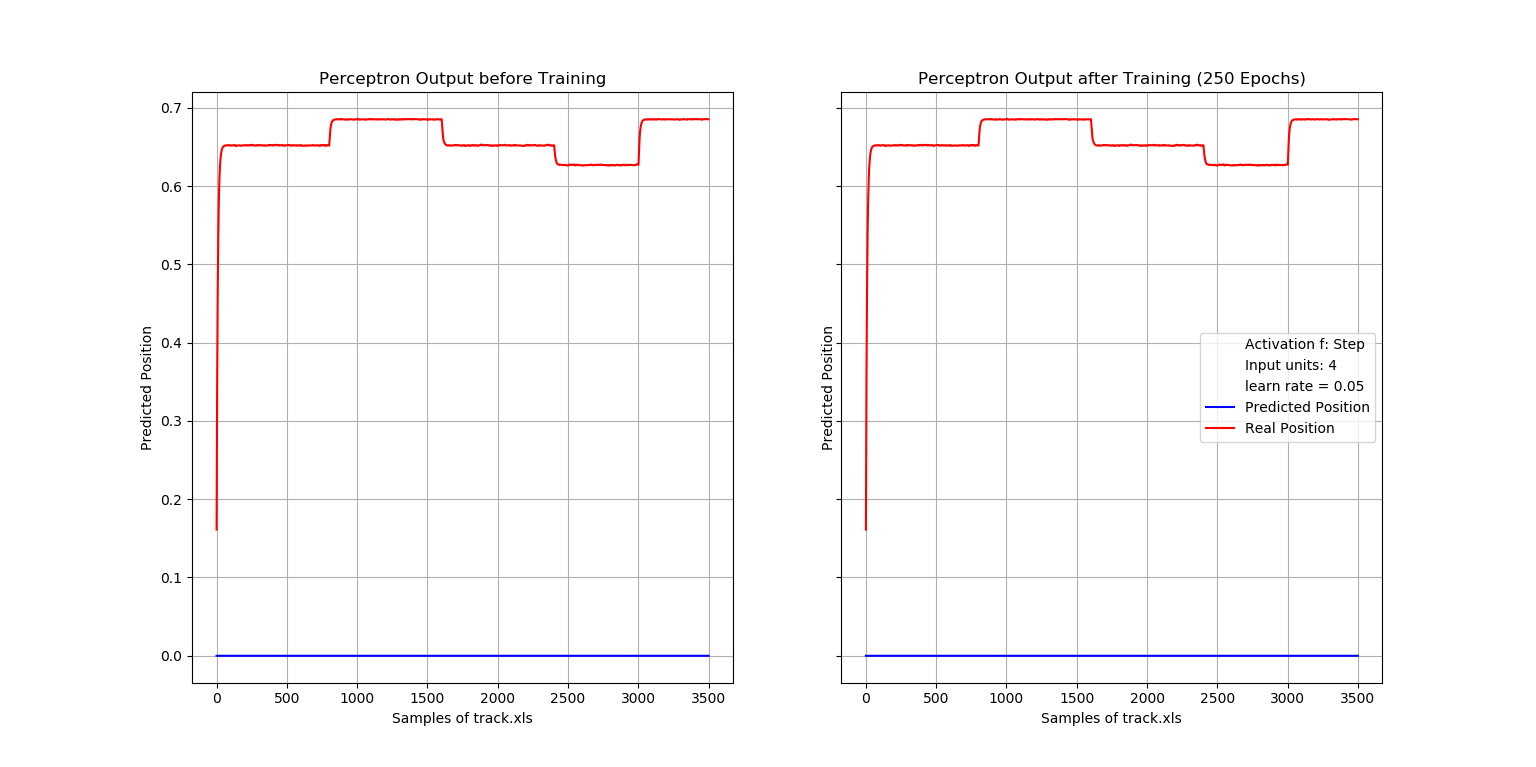
\includegraphics[width=14cm]{my_images/task2_perceptron_bfr_aftr.png}
	\end{center}
	\caption{Output of a perceptron with a step function before and after learning.}
	\label{fig:perceptron-bfr-aftr}
\end{figure}

\task{\textbf{c ) Replace the activation function with a logistic sigmoid. Show that the neuron is now capable of learning. Explain Why?}}\\

The graphs of figure \ref{fig:neuron-bfr-aftr} show that the trained perceptron is able to predict positions after replacing its Heaviside step function with a logistic sigmoid. The neuron now is able to output continues numbers which allows us to calculate. In addition one can derive the sigmoid function.

\begin{figure}[htbp]
	\subfigure[The perceptrons average error over all samples is decreasing.]{\label{fig:neuron-learn}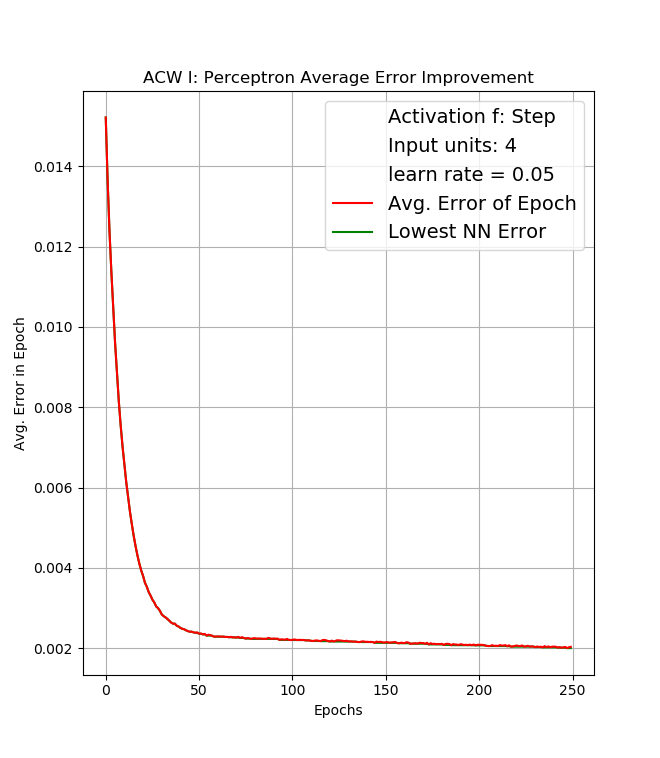
\includegraphics[width=0.432\textwidth]{my_images/task3_neuron_learn.png}}
	\subfigure[The predicted position of the perceptron is close to the real position of the sample data after training. ]{\label{fig:neuron-bfr-aftr}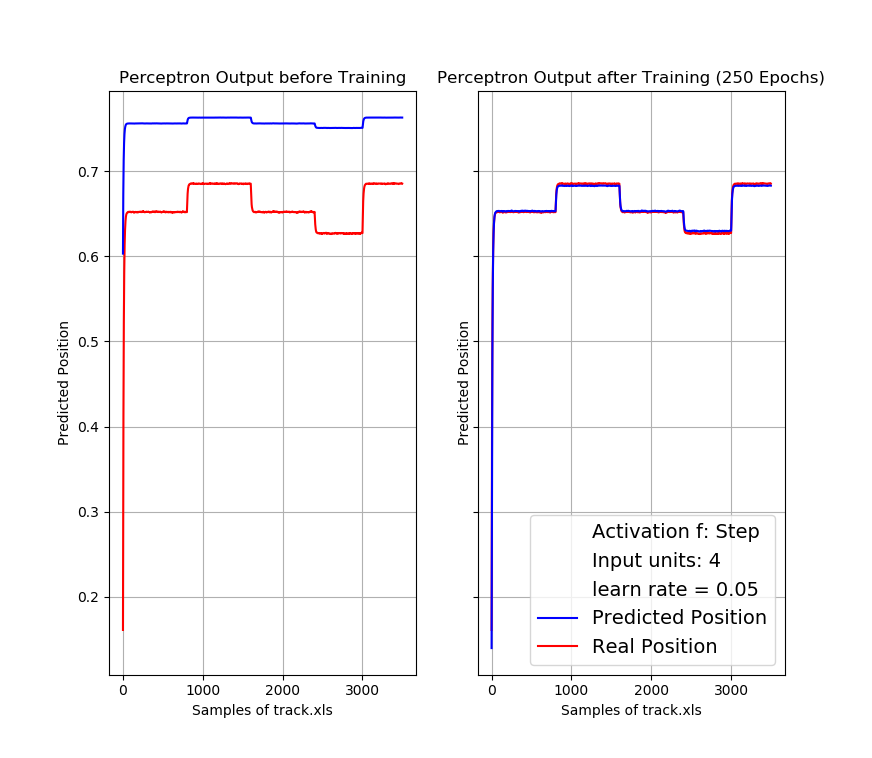
\includegraphics[width=0.568\textwidth]{my_images/task3_neuron_bfr_aftr.png}}
	\caption{Learning curve and outputs of a perceptron with a sigmoid activation function.}
	\label{fig:neuron}
\end{figure}

\task{\textbf{d ) Your write-up must include the code, diagrams for modeling the neuron(s), and any other information useful for your conclusions. You would also need to explain, how you would test the agent for unseen data, i.e explain whether it is able to generalize or not.}}\\

\task{\textbf{e ) In the data set there are a number of step changes. Note the steady state value of the data to identify the desired position. Use this value as the desired position (refer to lecture notes), and as many past values as you feel you need to predict the next position of the mouse.}}\\

\task{\textbf{f ) You should test you training by plotting \texttt{X(n)} and \texttt{X\_p(n)} (to get similar plots as above). You will find that there is a lag ? think why this is the case and report on it.}}\\

\task{\textbf{g ) Discuss possible ways you could predict both position and velocity, either using a perceptron (or a set of perceptrons) or a multi-layered network.}}\\


\end{document}

